\subsection{可解释性与错误分析}
\label{sec:interpretability}

能提高数字的重排序器是有用的。能解释其决策的重排序器在医学场景中是必要的，因为临床医生可能需要核实某段证据为何被提升。KCH-MedRank 的设计让 LambdaMART 特征重要性分数和超图通路使每一次排序决策都可追溯。本节给出量化证据，然后以同等篇幅分析失败案例。

\subsubsection{证据救回的三类机制}

KCH-MedRank 在留出测试集上将 661 个金标准段落从 Hybrid RRF top-10 之外救回 top-10（表~\ref{tab:failure-analysis-summary}）。我们对其中的 648 个按主导超图机制做了分类；其余 13 个虽被救回但未明确落入三类中的任何一类，不纳入以下细分。

MeSH 层级路径占救回的 75.9\%，平均排名提升 +22.1 位。问题与金标准段落通过 MeSH 树形祖先路径共享概念。询问 DITPA 的问题与关于甲状腺激素的段落，通过共享 MeSH 术语"甲状腺激素"及其树形祖先连接。

共享实体簇路径占救回的 23.9\%，平均提升 +14.0 位。金标准段落与其他高排名候选段落共享生物医学实体，共享实体超边簇通过扩散传播排序信号。

PrimeKG 关系路径占救回的 0.2\%。问题实体通过 PrimeKG 生物医学关系与段落实体相连（如"Dasatinib --治疗-- 白血病"）。低占比反映了 PrimeKG 中精确名称映射的稀疏性。

\begin{table}[t]
\centering
\small
\caption{可解释性量化：648 个可分类金标准段落的三种机制分类（661 个总救回段落中，13 个未明确归入单一主导机制）。每例按激活特征分数归入主导超图机制。}
\label{tab:interpretability-mechanisms}
\begin{tabular}{lrrr}
\toprule
Mechanism & Count & \% & Avg Rank Gain \\
\midrule
MeSH Hierarchy Path & 492 & 75.9 & +22.1 \\
Shared Entity Cluster Path & 155 & 23.9 & +14.0 \\
PrimeKG Relation Path & 1 & 0.2 & +25.0 \\
\cmidrule{1-4}
Total & 648 & 100.0 & +20.3 \\
\midrule
\multicolumn{4}{c}{\textit{Mechanism Activation Statistics (mean features per case)}} \\
\midrule
 & MeSH Hier. & Entity Clus. & Relation \\
\midrule
mesh\_overlap\_count & 1.18 & 0.03 & 0.00 \\
entity\_overlap\_count & 0.09 & 0.48 & 0.00 \\
question\_entity\_coverage & 0.06 & 0.36 & 0.00 \\
shared\_mesh\_parent\_size & 48.85 & 15.05 & 0.00 \\
shared\_entity\_edges & 126.59 & 127.84 & 128.00 \\
\bottomrule
\end{tabular}
\end{table}

\begin{table}[t]
\centering
\small
\caption{Mechanism co-occurrence in rescued cases. 89.2\% of rescues involve at least two concurrent knowledge pathways.}
\label{tab:mech-cooccurrence}
\begin{tabular}{lrr}
\toprule
Active Mechanisms & Count & \% \\
\midrule
MeSH Hierarchy + Entity Cluster + Relation & 256 & 39.5 \\
MeSH Hierarchy + Entity Cluster & 322 & 49.7 \\
Entity Cluster + Relation & 38 & 5.9 \\
Entity Cluster only & 32 & 4.9 \\
\bottomrule
\end{tabular}
\end{table}


表~\ref{tab:interpretability-mechanisms} 给出了分类结果。值得关注的是，89.2\% 的救回涉及至少两条并发知识路径，39.5\% 同时激活了全部三条。没有单一机制独立主导。这与结构消融一致：移除整个医学知识模块会导致超图退化回噪声，恰恰因为约束是协同工作的。

\begin{table}[t]
\centering
\small
\caption{943 个成对留出测试问题上增强 Hybrid w122 与增强 KCH-MedRank 的 top-10 失败分析。}
\label{tab:failure-analysis-summary}
\begin{tabular}{lr}
\toprule
诊断项 & 数值 \\
\midrule
成对问题数 & 943 \\
救回金标准证据的问题数 & 414 \\
救回金标准证据段落数 & 661 \\
丢失金标准证据的问题数 & 214 \\
丢失金标准证据段落数 & 307 \\
净救回段落数 & +354 \\
\bottomrule
\end{tabular}
\end{table}



\subsubsection{成功与失败案例}

理解方法在哪里失败，至少和庆祝它的成功同等重要。表~\ref{tab:failure-analysis-summary} 分类了 KCH-MedRank 未能救回的情况。

\begin{table}[t]
\centering
\small
\caption{BioASQ 留出测试集中 Enhanced Hybrid w122 与 KCH-MedRank 对比的代表性救回与丢失证据案例。}
\label{tab:case-study}
\begin{tabularx}{\linewidth}{p{0.12\linewidth}p{0.13\linewidth}X}
\toprule
案例 & 金标准排名 & 问题、信号与解释 \\
\midrule
救回 & 54 $\rightarrow$ 1 & 问题：What is the p-crAssphage? 主要信号包括 bacteriophages、crAssphage、viral genome 和 phylogeny。金标准段落与问题共享 bacteriophage 概念，并连接到局部 phage 相关候选簇，使重排序器能够恢复增强混合排序遗漏的证据。 \\
丢失 & 2 $\rightarrow$ 18 & 问题：Is there any protein that undergoes both mono-ubiquitination and poly-ubiquitination? 主要信号包括 ubiquitin、ubiquitination、ubiquitins 和 post-translational processing。该段落相关，但使用了相关生化形式和更宽泛的加工概念；同义词与层级特征未能充分对齐 mono-/poly-ubiquitination 与段落证据。 \\
\bottomrule
\end{tabularx}
\end{table}


\begin{figure}[htbp]
\centering
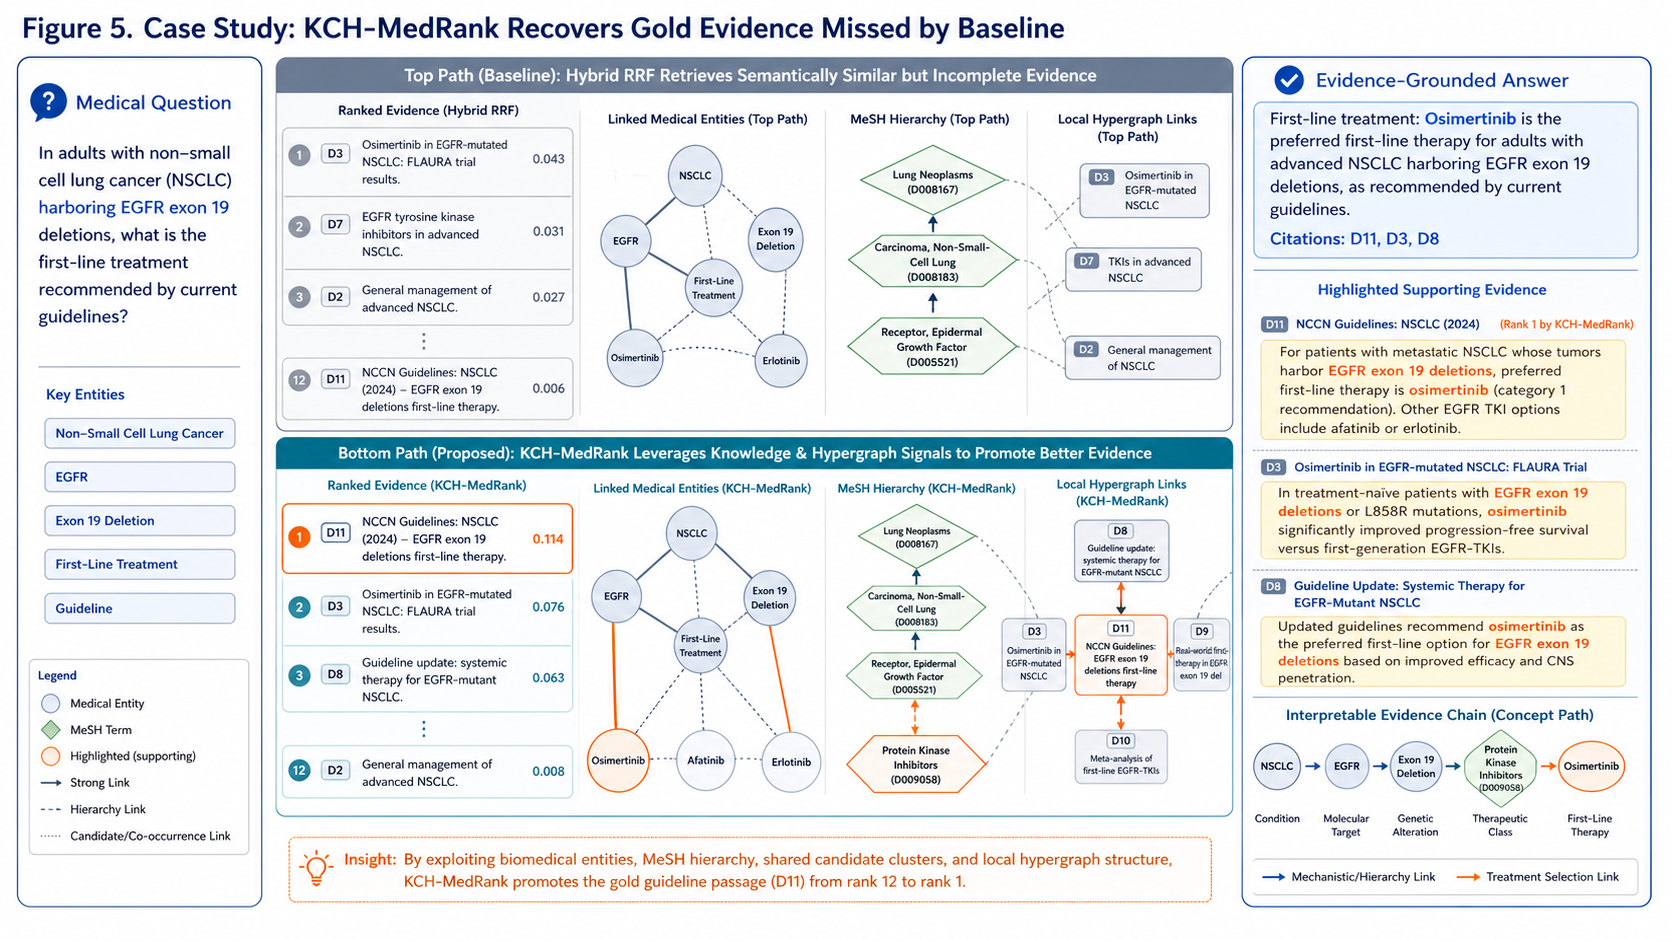
\includegraphics[width=0.98\linewidth]{figures/gpt_image2_figure_05.png}
\caption{案例分析示意图：KCH-MedRank 通过生物医学实体、MeSH 层级、共享候选簇和局部超图链接提升证据。}
\label{fig:gpt-case-study}
\end{figure}

最强的救回案例涉及 p-crAssphage，排名提升 +56 位。一篇关于噬菌体生物学的金标准段落从第 54 位升至第 1 位。主要对齐信号是共享的噬菌体概念，由局部噬菌体相关候选簇支撑。MeSH 和超图特征提升了医学上对齐的证据，即便增强混合排序已将其埋在前 10 之外。

最强的 MeSH 层级救回将关于 cGAS 通路的段落提升了 +83 位。问题"cGAS 通路的功能是什么"与竞争候选共享多个免疫学 MeSH 术语。一个密集的层级簇形成，超图扩散有效地传播了它。

失败案例围绕一个共同模式聚集。在丢失的泛素化案例中，一篇关于单泛素化和多泛素化 LDH 的金标准段落从第 2 位跌至第 18 位。问题和段落使用了相关的生化术语，但同义词和层级特征无法跨越表面形式连接到更广泛的翻译后加工概念。类似的丢失还出现在甲状腺激素类似物（DITPA 变体未被 MeSH 同义词覆盖）、cilengitide 受体（整合素术语不一致）、dasatinib 治疗（药物-适应症映射缺口）、GIST 治疗（罕见病概念覆盖稀疏）和 Fanconi 贫血（DNA 修复通路同义词失败）等案例上。每一个丢失案例都指向同一个未来方向：处理同义词和缩写的生物医学概念归一化将填补最大的剩余缺口。

\subsubsection{可解释性证据的说明}

三机制分析为 KCH-MedRank 的决策遵循医学通路这一说法提供了量化支撑。

每一条救回的段落至少激活了一个知识特征组。纯扩散驱动的救回为零。MeSH 层级路径是最频繁的主导通路，占 75.9\%。多条并发知识通路活跃于 89.2\% 的救回中。MeSH 驱动救回的平均排名提升远大于实体驱动（+22.1 vs.\ +14.0），表明层级概念对齐比扁平实体共现携带了更多的排序信号。

一个方法学上的提醒：机制分类使用的是 LambdaMART 消费的同一组特征分数。它识别的是哪些特征最强烈激活，而非哪些因果驱动排序。像 SHAP 这样的因果归因方法可以在未来工作中强化这一声明。
